\documentclass[11pt]{article}
\usepackage{graphics,epsfig,amsmath,amssymb}
\usepackage{epsf}
\usepackage{boxedminipage}
\usepackage{fullpage}
\usepackage{fancyheadings}
\usepackage{times}
\usepackage{amsmath}
\usepackage{ifthen}
%\usepackage{pseudocode}
\usepackage{psfrag}
\pagestyle{fancy}

\setlength{\topmargin}{.2in}
\setlength{\parindent}{0in}
\setlength{\parskip}{.15in}
\setlength{\footskip}{0.1in}

\newcounter{pctr}
\stepcounter{pctr}

\newcounter{partctr}

\newcommand{\ie}{{\em i.e.}}
\newcommand{\eg}{{\em e.g.}}

\newcommand{\ch}{\item {\bf True~~/~~False~~}}
\newcommand{\tfnote}{\probnote{Circle True or False for each choice.}}
\newcommand{\allapply}{\probnote{Circle ALL that apply}}
\newcommand{\bestanswer}{\probnote{Circle the BEST answer}}
\newcommand{\ansbelow}{\probnote{Answer legibly in the space below.}}

\renewcommand{\thesection}{{\bf\Roman{section}}}
\renewcommand{\theenumi}{{\bf\Alph{enumi}.}}
\renewcommand{\labelenumi}{{\bf\Alph{enumi}.}}

\newcommand{\setversion}[1]{\def\version{#1}}
%\setversion{answers}
\setversion{quiz}

\ifthenelse{\equal{\version}{answers}}{
    \newcommand{\sols}[1]{#1}
}{
    \newcommand{\sols}[1]{}
}


\begin{document}

\newcounter{answer}
\newenvironment{answer}[1][\relax]{\refstepcounter{answer}\begin{list}%
 {}{\leftmargin 0pt\rightmargin 0pt\labelsep 3pt\parsep 0pt%
 \setlength{\listparindent}{\parindent}}
    \item {\bf Answer \theanswer #1}\
    }{\hspace*{\fill}$\blacksquare$\end{list}} 



% uses these macros to delimit problems
\newcommand\prob[1]%
  {\begin{itemize}\item[]%
   \vspace{.2in}{\bf\thepctr. ~[#1~ points]:}\stepcounter{pctr}}
\newcommand\eprob{\end{itemize}}
\newcommand\probnote[1]%
  {\\\begin{tabular}{cr} \hspace{3in} & {\bf (#1)} \\ \end{tabular}}

% headers/footers
\lhead[\fancyplain{}{\bf Page \thepage ~of \pageref{lastpage}}]%
      {CS 6250 Fall 2011, Quiz 2}
\lfoot[{\bf Name: }]%
      {{\bf Name: }}
\rhead[CS 6250 Fall 2011, Quiz 2]%
      {\fancyplain{}{\bf Page \thepage ~of \pageref{lastpage}}}
\cfoot{}
%\setlength{\headrulewidth}{0in}
\setlength{\headsep}{.3in}

 % Compact itemize and enumerate.  Note that they use the same counters and
% symbols as the usual itemize and enumerate environments.
\def\compactify{\itemsep=0pt \topsep=0pt \partopsep=0pt \parsep=0pt}
\let\latexusecounter=\usecounter
\newenvironment{CompactItemize}
  {\def\usecounter{\compactify\latexusecounter}
   \begin{itemize}}
  {\end{itemize}\let\usecounter=\latexusecounter}
\newenvironment{CompactEnumerate}
  {\def\usecounter{\compactify\latexusecounter}
   \begin{enumerate}}
  {\end{enumerate}\let\usecounter=\latexusecounter}


\cfoot{}
\pagestyle{empty}

\begin{center}
\begin{tabular}{lr}
\resizebox{1in}{!}{\includegraphics{GT}}
&
\parbox{4in}{
    {\Large\it College of Computing} \\ \\
    {\LARGE\sf Georgia Institute of Technology} 
}
%
\end{tabular}
\end{center}

\begin{center}
{\Large{\bf CS 6250: Computer Networking: Fall 2011} \\
 \vspace{.15in} \Huge{\bf Quiz II}} 
%\vspace{.2in}

% this is the box on the first page with overall quiz information
\begin{boxedminipage}[h]{6in}
There are \underline{14 questions} (and one bonus question) and
  \underline{\pageref{lastpage} pages} in this quiz booklet (including
  this page).  Answer each question according to the instructions given.
  You have {\bf 85 minutes}.

%\vspace{.1in} The last page is an easy question.  {\em Rip this
%page off of your exam for five bonus points.}  Turn it in anonymously if
%you like.


\vspace{.1in} 
If you find a question ambiguous, write down any
assumptions you make.  {\bf Be neat and legible.}  If I can't
understand your answer, I can't give you credit!  There are three pretty
challenging questions (clearly marked); you may want to look through the
whole quiz and save those for last.

\vspace{.1in} 
Use the empty sides of this booklet if you need scratch space.  You
may also use them for answers, although you shouldn't need to.  {\em If you
do use the blank sides for answers, make sure to clearly say so!}

\vspace{.1in} 
{\bf Note well: Write your name in the space below AND your initials at the bottom of each
page of this booklet.}

\begin{center}{\bf THIS IS AN ``OPEN NOTES, OPEN PAPERS'' QUIZ.\\
LAPTOPS ARE ALLOWED, BUT ONLY FOR REVIEWING PAPERS AND NOTES \\
NO OTHER MATERIALS, NO PHONES, NO PDAS.\\
{\em ABSOLUTELY NO EMAIL OR MESSAGING OF ANY KIND!} \\
MAKE SURE YOU'VE READ ALL THE INSTRUCTIONS ABOVE!}
\end{center}
{\em Initial here to indicate that (1)~you've read the instructions and (2)~
you agree to abide by the Georgia Tech Honor Code: }

\vspace{.1in} The last page has easy bonus questions, which you can
answer outside of the allotted time.  Rip the last page off of your
quiz for five bonus points.  Turn it in anonymously if you like.

\end{boxedminipage}
\end{center}
\vspace*{0.25in}
\begin{center}
{\it Do not write in the boxes below}
\end{center}

\begin{center}
\begin{tabular}{|l|l|l|l|l|l|l|l|l|} \hline \hline
{\bf 1-5 (xx/20)}& {\bf 6-7 (xx/13)} & {\bf 8-11 (xx/24)} & {\bf 12-14
  (xx/13)} &{\bf Bonus (5+xx)} & {\bf Total 
  (xx/70)}  \\ \hline 
 & & & & & \\ 
 & & & & & \\ \hline \hline
\end{tabular}
\end{center}

\vspace{.2in}
{\bf\Large{Name:}}

\newpage
\pagestyle{fancy}

\section{Warmup}

\prob{4} Which of the following is true about measurements of an ISP
access link performed from the home gateway router that is directly
connected behind the DSL or cable modem? 
\allapply

\setcounter{partctr}{0}
\begin{list}{\bf\Alph{partctr}.}{\usecounter{partctr}}
\item A single-threaded TCP throughput measurement should be able to
  accurately measure the full capacity of an access link that has high
  packet loss, if the size of the upload or download is large enough.
\item The router can monitor the network for other activity and only
  perform measurements when other network traffic is low.
\item Wireless interference inside the home may affect the performance
  measurements of the access link.
\item When DSL ``interleaving'' is applied to the access link,
  the latency to the first router in the upstream ISP's network
  should be equal to about the propagation delay of the packet.
\item All of the above.
\end{list}
\eprob

\sols{
\begin{answer}
The answer is: (B).
\end{answer}
}


\prob{4} Which of the following are true about virtual networks?
\allapply
\setcounter{partctr}{0}
\begin{list}{\bf\Alph{partctr}.}{\usecounter{partctr}}
%\begin{enumerate}
\item Virtual networks that share the same physical infrastructure must
  not have overlapping IP address space.
\item A virtual link in a virtual network can traverse multiple physical
  routers. 
\item An MPLS tunnel is an example of a virtual link.
\item A virtual router that is implemented fully in software must have
  its forwarding tables in ``user space'', as described in the VINI
  paper. 
\item None of the above.
\end{list}
\eprob

\sols{
\begin{answer}
The answer is: (B), (C).
\end{answer}
}

\prob{4} Which of the following are true of data center networks?
\bestanswer
\setcounter{partctr}{0}
\begin{list}{\bf\Alph{partctr}.}{\usecounter{partctr}}
%\begin{enumerate}
\item Designers of data center networks often aim to address nodes in a
  ``flat'' layer two Ethernet topology to make it easier to migrate
  servers from one part of the network to another.
\item Layer two addressing cannot scale to the size of an entire data
  center because every switch must store forwarding table entries for
  every server in the network.
\item In PortLand, servers send broadcast ARP queries to discover the
  MAC address of a server with a certain IP address.
\item In VL2, servers send broadcast ARP queries to discover the MAC
  address of a server with a certain IP address.
\item None of the above
\end{list}
\eprob

\sols{
\begin{answer}
The answer is (A), (C).
\end{answer}
}

\newpage
\prob{4} Which of the following are true about 802.11 wireless networks?
\allapply
\setcounter{partctr}{0}
\begin{list}{\bf\Alph{partctr}.}{\usecounter{partctr}}
%\begin{enumerate}
\item Without RTS/CTS, two senders could send packets that collide at
  the same receiver.
\item Enabling RTS/CTS could prevent a sender from sending a packet,
  even if sending the packet would not have caused a collision at the receiver.
\item Losses at the 802.11 link layer might be observed as higher
  latencies with a tool like ICMP ping.
\item A sender can use a CTS to reserve the data channel for itself.
\item None of the above.
\end{list}
\eprob

\sols{
\begin{answer}
The answer is: (A), (C), (D).
\end{answer}
}


\prob{4} Which of the following features have spammers exhibited that
are different than legitimate senders?  \allapply
\setcounter{partctr}{0}
\begin{list}{\bf\Alph{partctr}.}{\usecounter{partctr}}
%\begin{enumerate}
\item Sending messages of similar sizes to many different recipients
\item Sending messages from hijacked IP address space
\item Sending messages from network ranges that contain a large number
  of mail servers
\item Sending messages that exhibit some ``geographic locality'' (i.e.,
  the messages don't tend to travel further than a certain distance to
  their receiver).
\item All of the above
\end{list}
\eprob

\sols{
\begin{answer}
The answer is: (E).
\end{answer}
}




\newpage
\section{Wireless Networking}

\prob{6}
Consider a device that wants to transmit data over the recently de-regulated
wireless spectrum ``white space'', as in Murty's {\em White Space
  Networking with Wi-Fi like Connectivity}. 
\setcounter{partctr}{0}
\begin{list}{\bf\Alph{partctr}.}{\usecounter{partctr}}
\item What are the benefits to transmitting data in the white space
  spectrum, as opposed to the 2.4 Ghz or 5 GHz ISM bands that current
  WiFi devices use today?
\item Give two reasons why transmission in white spaces is more
  complicated than trasnmission in the ISM bands.
\item Explain the tradeoff between performance and contention that the
  access point faces when selecting the width of spectrum to reserve for
  communication with the device. 
\end{list}
~\ansbelow 
\vspace{2in}
\eprob

\sols{
\vspace{-1in}
\begin{answer}
\end{answer}
}


\newpage

\prob{7} Consider the figure below, which shows packet {\em loss rates} for each
wireless ``link''.  {\em Show your work below.}
%% ADD FIGURE
\begin{center}
\resizebox{0.5\textwidth}{!}{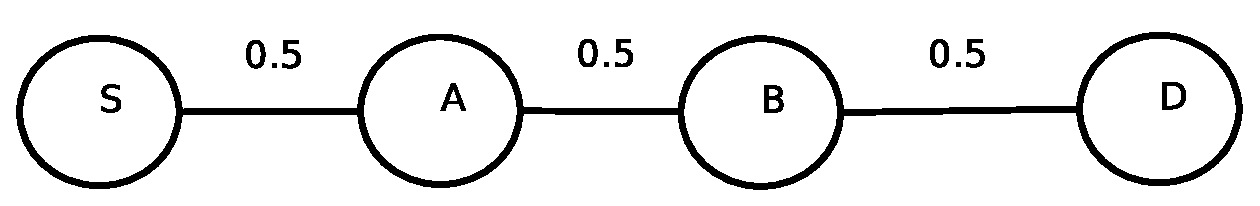
\includegraphics{exor}}
\end{center}
\setcounter{partctr}{0}
\begin{list}{\bf\Alph{partctr}.}{\usecounter{partctr}}
\item (3 points) Assuming that each packet is transmitted hop-by-hop, what is the
  {\em total}   expected number of transmissions for a packet to reach
  node $D$ from node $S$?
\item (4 points) Suppose that, with probability $0.5$ node $B$ hears the {\em
  initial} transmission from node $S$, and that node $B$ will
  re-transmit the packet from node $S$ if it hears it (as in the ExOR
  paper).  What is the expected number of transmissions for the packet
  to reach node $B$, and what is the total expected number of transmissions
  for the packet to reach node $D$?  ({\em Hint:} You must consider two
  cases when considering your probabilities: the case where the
  transmission from node $S$ reaches $B$ and the case where it does not.)
\end{list}
~\ansbelow 
\vspace{3in}
\eprob

\sols{
\begin{answer}
\end{answer}
}



\newpage
\section{Performance and Security}

\prob{5} Explain the difference between {\em persistent} HTTP
connections and {\em pipelined} HTTP connections.  Explain how each of
these optimizations can reduce the overall page load time for a Web page.~\ansbelow
\vspace*{2.5in}
\eprob

\prob{5} Describe one advantage and one disadvantage of using {\em content
filters} for spam filtering.  Describe one advantage and one disadvantage
of using {\em IP blacklists} for spam filtering.
\vspace*{2.5in}
\eprob


%% \prob{8} Two factors that are causing routing
%% table growth in modern routing tables are multihoming and prefix hijack
%% prevention. Explain how an operator could use additional prefixes in the
%% Internet's routing table to (1)~control inbound traffic; and (2)~defend
%% against an incident where their own prefix is hijacked.
%% ~\ansbelow 
%% \vspace{3in}
%% \eprob


\newpage
\prob{8}
In Problem Set~2, you studied the mechanics of traffic shaping.  {\em
  PowerBoost} is a feature advertised by cable ISPs such as
Comcast. Customers with PowerBoost enabled get a burst of traffic at a
rate higher than the service plan rate for a limited duration.  

Token bucket filters, such as the one you studied in Problem Set~2, are
commonly used to implement PowerBoost.  Each customer has a dedicated
token bucket filter that regulates traffic to that customer.  Consider a
Comcast customer whose connection is capable of a maximum rate of $20$
Mbits$/$s.

\setcounter{partctr}{0}
\begin{list}{\bf\Alph{partctr}.}{\usecounter{partctr}}
\item This customer purchases a basic $6$~Mbits$/$s plan {\em without}
  PowerBoost. What is the configured token rate and bucket size?

\item The customer upgrades to a $12$ Mbits$/$s plan, with the
  capability for PowerBoost at line rate (20 Mbits/s).  PowerBoost rates
  apply for the first 10~MBytes (80~Mbits) of traffic. What is the
  duration of PowerBoost? What is the configured token rate and bucket
  size?

\item Due to a misconfiguration at the headend, the token rate is set to
  $25$~Mbits$/$s.  The bucket size is unchanged. What is the burst size,
  burst duration, and the long-term average throughput that this
  customer obtains?
\end{list}
~\ansbelow 
\vspace*{1.5in}
\eprob

\newpage
\prob{6} Consider the following DNS lookup, issued from a machine at
Georgia Tech, output from running {\tt dig} on {\tt
  static.ak.fbcdn.net}, the domain name for Facebook's content
distribution network:

%% % dig static.ak.fbcdn.net

%% ; <<>> DiG 9.6.0-APPLE-P2 <<>> static.ak.fbcdn.net
%% ;; global options: +cmd
%% ;; Got answer:
%% ;; ->>HEADER<<- opcode: QUERY, status: NOERROR, id: 17166
%% ;; flags: qr rd ra; QUERY: 1, ANSWER: 4, AUTHORITY: 0, ADDITIONAL: 0

%% ;; QUESTION SECTION:
%% ;static.ak.fbcdn.net.		IN	A



\begin{scriptsize}
\begin{verbatim}
;; ANSWER SECTION:
static.ak.fbcdn.net.	7185	IN	CNAME	static.ak.facebook.com.edgesuite.net.
static.ak.facebook.com.edgesuite.net. 21586 IN CNAME a749.g.akamai.net.
a749.g.akamai.net.	15	IN	A	208.44.23.43
a749.g.akamai.net.	15	IN	A	208.44.23.34
a749.g.akamai.net.	15	IN	A	208.44.23.50
a749.g.akamai.net.	15	IN	A	208.44.23.48
a749.g.akamai.net.	15	IN	A	208.44.23.35
a749.g.akamai.net.	15	IN	A	208.44.23.27
a749.g.akamai.net.	15	IN	A	208.44.23.64
;; Query time: 4 msec
;; SERVER: 8.8.8.8#53(8.8.8.8)
;; WHEN: Wed Nov 30 15:59:35 2011
;; MSG SIZE  rcvd: 224
\end{verbatim}
\end{scriptsize}

\setcounter{partctr}{0}
\begin{list}{\bf\Alph{partctr}.}{\usecounter{partctr}}
%\item What is the purpose of the two CNAME entries?  
\item How long would the IP address corresponding to this domain name
  remain in a DNS resolver's cache?  
\item Why does the query return multiple ``A'' records to a single client?
\item A ping to these IP addresses indicates that these
  servers are approximately 2 milliseconds away from Georgia Tech.  A
  similar DNS lookup from a machine at MIT in Boston, Massachusetts
  returns IP addresses in {\tt 18.7.20/24}, less than a millisecond
  away from the machine at MIT that issued the query.
\begin{itemize} 
\item Why do different DNS clients receive different A record answers for the same DNS
  lookup? 
\end{itemize}
\end{list}
~\ansbelow 
\vspace{3in}
\eprob


\newpage
\section{Accelerating Web Performance}

George Burdell has been noticing that his Web performance to many
popular Web sites is slower than he would like.  For some sites, he's
noticed that download times can be more than half a second, even for
relatively small Web pages.  He has asked three of his friends to
compare download times to nine popular Web sites, as well.  The download
times in milliseconds are shown in the stacked bar plot below.  Each bar
represents one of the four users, and the total time can be computed by
adding the the
following mututally exclusive components:
\begin{itemize}
\itemsep=-1pt
\item {\em Lookup Time:} The time to resolve the DNS name for the site. 
\item {\em Connect Time:} The time to complete the TCP three-way handshake.
\item {\em Transfer Start Time:} The time until the first byte is received at
  the client.
\item {\em Transfer Time:} The time for the transfer to complete.
\end{itemize}
\begin{center}
\resizebox{0.8\textwidth}{!}{\includegraphics{web-latencies}}
\end{center}
%% \prob{3} Why might the time to resolve a DNS query differ for different users?  Why
%% might the time to resolve a DNS query differ for different Web sites?
%% ~\ansbelow 
%% \vspace{2in}
%% \eprob
\prob{3} George notices that, in many cases, the
transfer time is not the only significant contributor to the overall
page load time.  He looks at this data and says: ``Upgrading to a higher
service plan would be a waste of money: Simply adding more throughput
isn't going to reduce some of the significant bottlenecks that are
slowing down my Web downloads.''  Is he right?  Why or why not?  (Which
components of the overall transfer time could be reduced with higher
throughput?)  ~\ansbelow
\vspace{2in}
\eprob

%% \prob{3} George notices that when he loads Facebook using Chrome, the
%% page loads more quickly than it does when he loads it in Firefox under
%% the same conditions.  What is one reason that he might be seeing
%% different performance with different browsers?
%% ~\ansbelow
%% \vspace{2in}
%% \eprob

\newpage
George ``pings'' {\tt www.facebook.com} and notices that round-trip
times to the Facebook server are about 30 milliseconds.  Suppose that
the Facebook page size is about 30 Kilobytes, that packet MTUs are 1
Kilobyte, that the initial TCP congestion window for Facebook is $4$
packets, that the connection leaves TCP slow start and starts AIMD
congestion control when window size is $8$ packets, and that there is no
packet loss or buffering.  (Assume no parallel HTTP connections.)

\prob{5} How many roundtrips and how many milliseconds will it take
to download the Facebook page, excluding the time for the TCP 3-way
handshake and server setup time?  {\em Show your work.}
~\ansbelow 
\vspace{2in}
\eprob

\prob{5} George says: ``30 milliseconds is really far away.  The
Facebook page would load much more quickly if I enabled a Web cache on
my home router, which is only 1 millisecond away.''  Suppose, for
simplicity, that half of the content on the Facebook page is cacheable,
so that 15 Kilobytes can be fetched from the home router cache (1
millisecond round trip) and 15 Kilobytes must be fetched from the
Facebook server (30 milliseconds round trip).  (Assume no
parallel HTTP connections.)
\begin{itemize}
\item How many milliseconds
will it take to fetch the cached content from the router?  
\item How many milliseconds
will it take to fetch the remaining content from the Facebook server?  
\end{itemize}
~\ansbelow 
\vspace{2in}
\eprob

\newpage
\prob{5} {\bf Bonus.} George realizes that, while caching some content
will help improve the performance for various Web sites, his Netflix
performance may still suffer.  Which performance metrics would be most
relevant for streaming, and what possible optimizations could George
consider on his home router to improve {\em streaming} performance?
(Keep in mind that George only controls the client side of the
connection.)
~\ansbelow 
\vspace{2in}
\eprob


\newpage
\section{Bonus: Anonymous Course Feedback}

{\bf This page is anonymous.}  Rip this off from your exam, and turn it
in separately if you like.  You'll get five points for simply ripping
off the last page of the exam, but I'd prefer if you fill it out and
hand it in in a separate stack.
\vspace{.5in}

What were the things you liked most about the course?  Anything is
fair game here (topics, course structure, board technique, etc.).
\vspace{1.5in}


What are the things you liked least about the course?  Again,
anything is fair game.
\vspace{1in}


If you could change one thing about the course in a future offering,
what would it be?
\vspace{1in}


If you could keep one thing about the course in a future offering,
what would it be?
\vspace{1in}




\label{lastpage}
\end{document}



